\documentclass[12pt, legalpaper]{exam}
\usepackage[utf8]{inputenc}
\usepackage[english]{babel}
\usepackage[margin=.8in]{geometry}
\usepackage{amsmath,amssymb}
\usepackage{multicol}
\usepackage{graphicx}
\usepackage{tikz}
\usepackage{lastpage}
\usepackage{tabularx}
\usepackage{hyperref}
\usepackage{tcolorbox}
\newcommand{\course}{Introduction to Optimization}
\newcommand{\term}{Fall 2023}
\newcommand{\examnum}{Report of Programming Task 1}


\begin{document}
\noindent \examnum \, of the  course ''\course'' - \term


\noindent
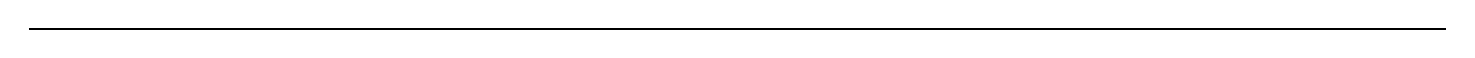
\begin{tikzpicture}
\draw[thick] (0,0) -- (18,0);
\end{tikzpicture}




\vspace{12pt}
\begin{center}
    \textbf{Report 1}
\end{center}
% \noindent \textbf{Requirements}

\vspace{12pt}

\noindent  \textbf{Team information.}

\begin{itemize}
    \item Team leader: Aleksandr Ryabov
    \item Team member 1: Aleksandr Ryabov
    \item Team member 2: Aleksandr Ryabov
    \item Team member 3: Aleksandr Ryabov
    \item Team member 4: Aleksandr Ryabov
    \item Team member 5: Aleksandr Ryabov
\end{itemize}
\vspace{12pt}
\noindent     \textbf{Link to the product.}
\begin{itemize}
    \item The product is available:  
\end{itemize}

\vspace{12pt}

\noindent  \textbf{Programming language.}
\begin{itemize}
    \item Programming language: Python
\end{itemize}

\vspace{12pt}

\noindent  \textbf{Linear programming problem.}
\begin{itemize}
\item Maximization or Minimization?
\\
Programm can solve both types of LPP. 
\vspace{10pt}
    \item Objective function: $F = 5x_1 + 4x_2 + 0x_3 + 0x_4 + 0x_5 + 0x_6$
    \vspace{10pt}
    \item Constraint functions:
    \begin{gather*}
        6x_1 + 4x_2 + x_3 = 24 \\
        1x_1 + 2x_2 + x_4 = 6  \\
        -1x_1 + 1x_2 + x_5 = 1 \\
        0x_1 + 1x_2 + x_6 = 2  \\
        x_1,...,x_6 \geq 0
    \end{gather*}
    \vspace{2cm}
\end{itemize}



\noindent     \textbf{Input}

\vspace{12pt}
The input contains:
\begin{itemize}
    \item Maximization or minimization problem
    \item A vector of coefficients of objective function - $A$.
    \item Size of the matrix of coefficients of constraint function - $m$ and $n$
    \item A matrix of coefficients of constraint function - $C$.
    \item A vector of right-hand side numbers - $b$.
    \item The approximation accuracy $approx$.
\end{itemize}

\vspace{12pt}
\textbf{Example of input:}
\begin{verbatim}
    1 
    
    5  4  0  0  0  0

    4  6

    6  4  1  0  0  0 
    1  2  0  1  0  0
    -1 1  0  0  1  0
    0  1  0  0  0  1

    24  6  1  2

    1.0000001
\end{verbatim}

\vspace{12pt}
\noindent     \textbf{Output/Results}

The output contains:
\begin{itemize}
    \item Messange with error and string "The method is not applicable!"
    
or
    \item Messange with programm success
    \item A vector of decision variables - $X^*$.
    \item Maximum (minimum) value of the objective function.
\end{itemize}

\vspace{12pt}
\textbf{Example of output:}

\begin{verbatim}
    ### Maximum achived ###

    ######################################
    ### ANSWER                         ###
    ### Vector of decision variables   ###
    ### Values of 'x' vector is [3.0, 1.5, 0, 0, 2.5, 0.5]
    ### Value of function is 21
    ### Programm finished successfully ###
    ######################################
\end{verbatim}

\noindent
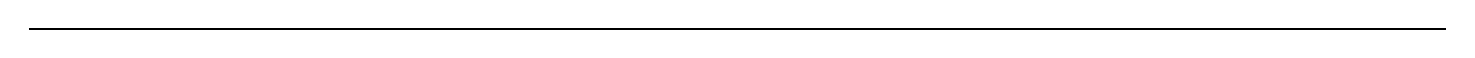
\begin{tikzpicture}
\draw[thick] (0,0) -- (18,0);
\end{tikzpicture}




\vspace{24pt}
\noindent     \textbf{Code}

Copy-paste your code here.


\end{document}
